
%%%%%%%%%%%%%%%%%%%%%%%%%%%%%%%%%%%%%%%%%%%%%%%%%%%%%%%%%%
\chapter{Introduction}
\label{chapter_introduction}
%%%%%%%%%%%%%%%%%%%%%%%%%%%%%%%%%%%%%%%%%%%%%%%%%%%%%%%%%%

\begin{figure}
\centering

\includegraphics[width=1.0\textwidth]{figures/intro/unilever_w_neg_space.pdf} 
\caption[Unilever packing and its negative space]
{\label{fig_logo_packing} 
\newtext
{
(a) Unilever packing that consists of 25 elements arranged inside a ``U'' container. \newline
(b) The red region is called negative space, which is the remaining area that is not claimed by the elements. 
}
}
\end{figure}

\begin{figure}
\centering
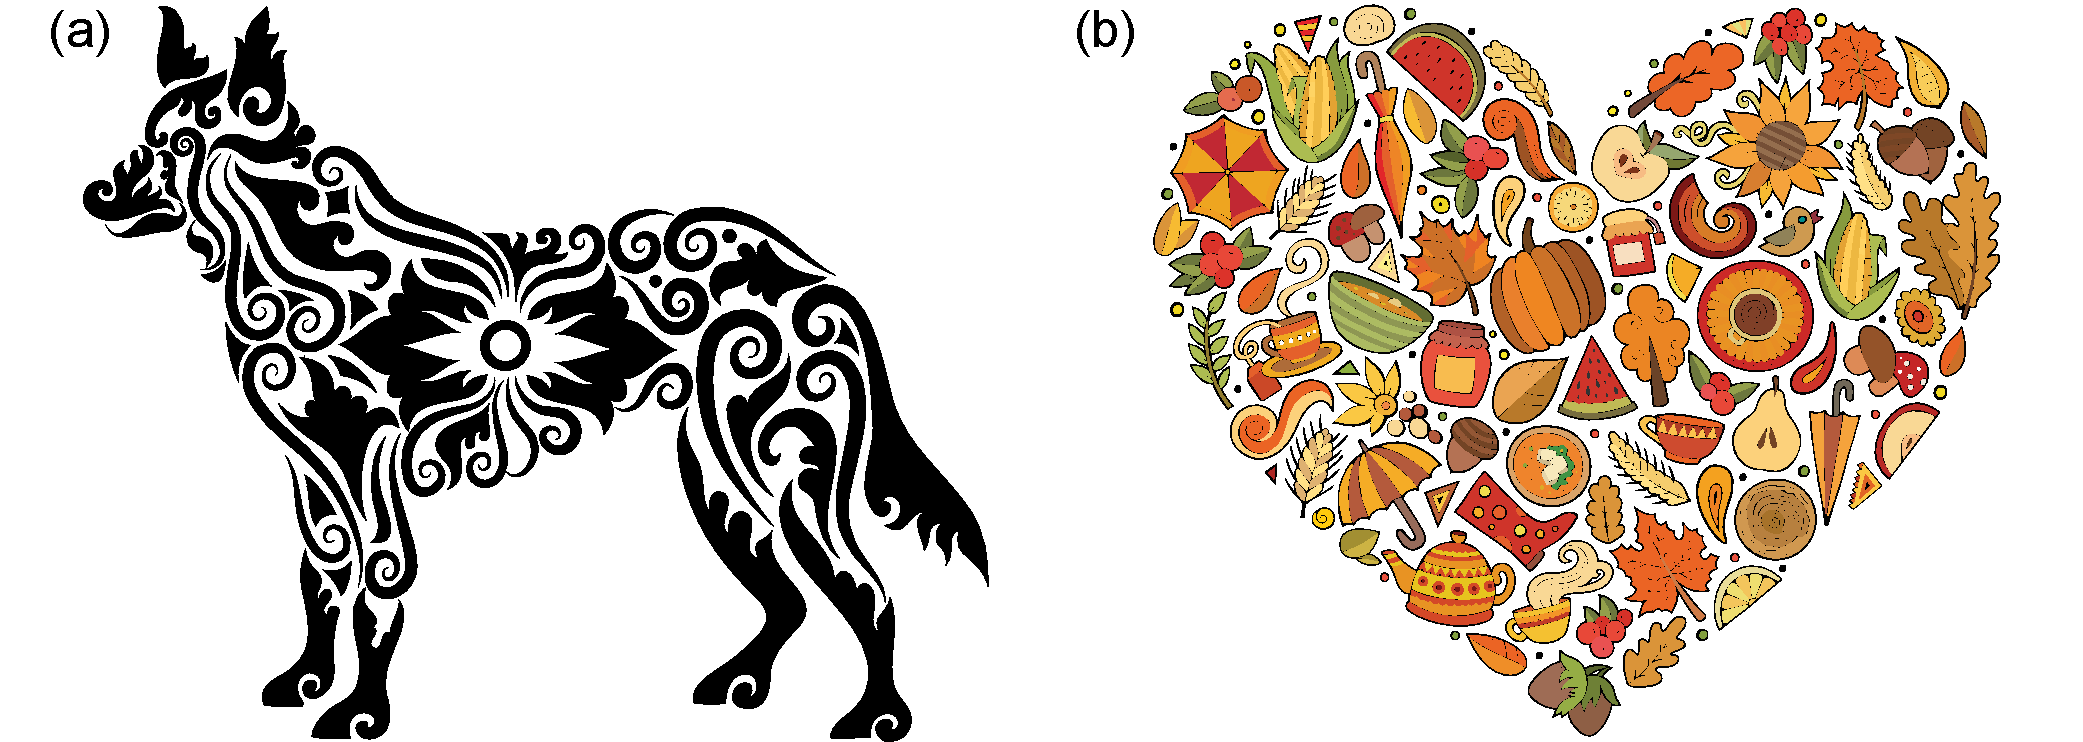
\includegraphics[width=1.0\textwidth]{figures/intro/balabolka_dog_flow.pdf} 
\caption[Packings in graphic design]
{\label{fig_graphic_designs} 
\newtext
{
(a) A packing of autumn-themed elements, created by Balabolka.
(b) A packing of abstract-shaped elements that create a flow visual style, created by ComicVector703.
}
 }
\end{figure}

\begin{figure}
\centering
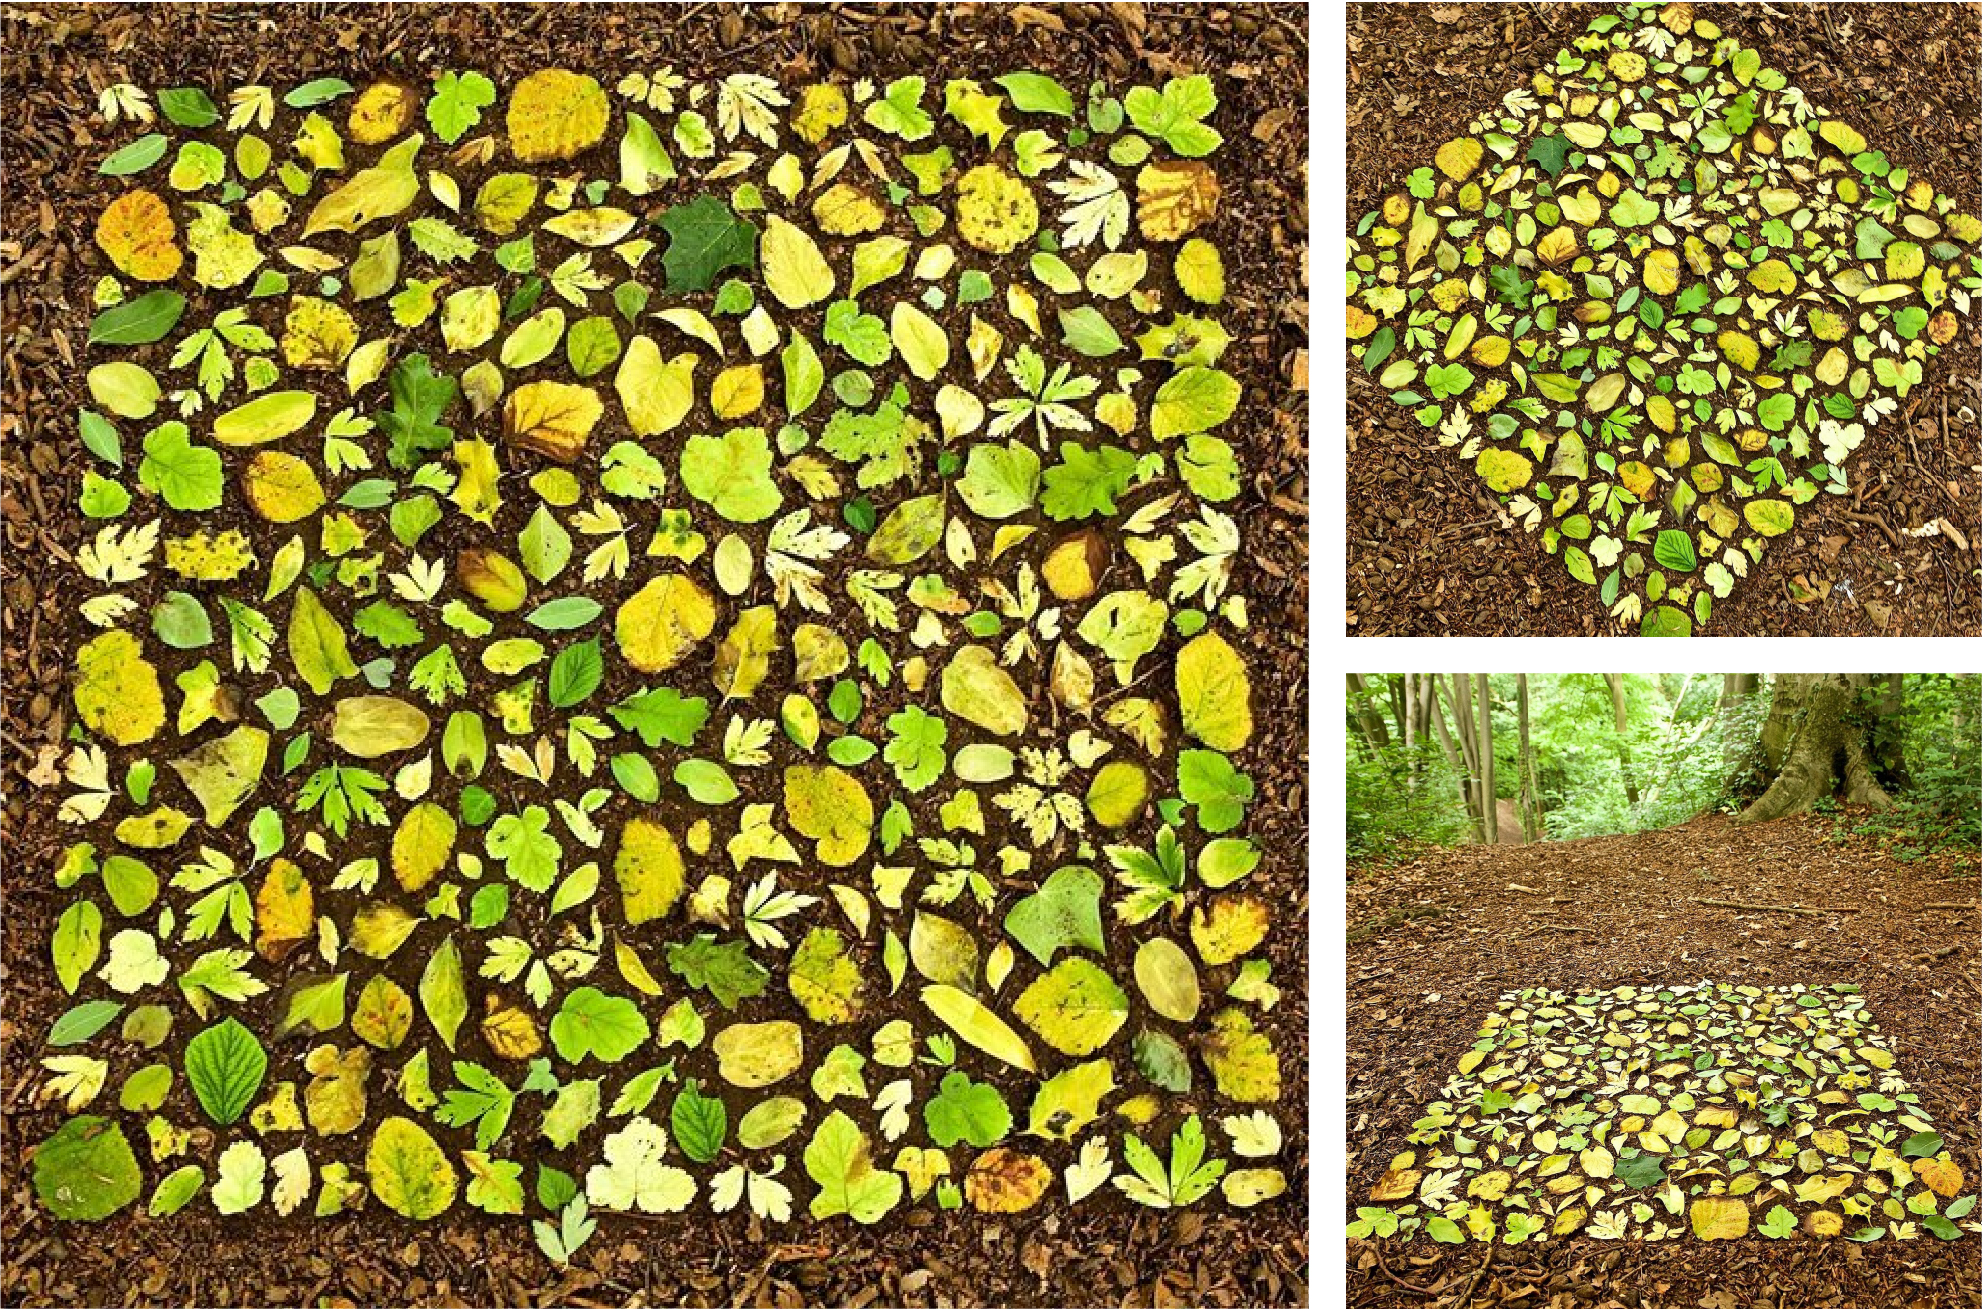
\includegraphics[width=1.0\textwidth]{figures/intro/woodland.jpg} 
\caption[A packing in art]
{\label{fig_woodland} 
\newtext
{
A packing of leaves by James Brunt. Each leaf is oriented toward the center of the circle.
}
 }
\end{figure}

%\begin{figure}
%\centering
%\includegraphics[width=0.5\textwidth]{figures/intro/valve_lobby.jpg} 
%\caption{\label{fig_valve_lobby} 
%A packing installation in a lobby of a video game company. }
%\end{figure}

%\begin{figure}
%\centering
%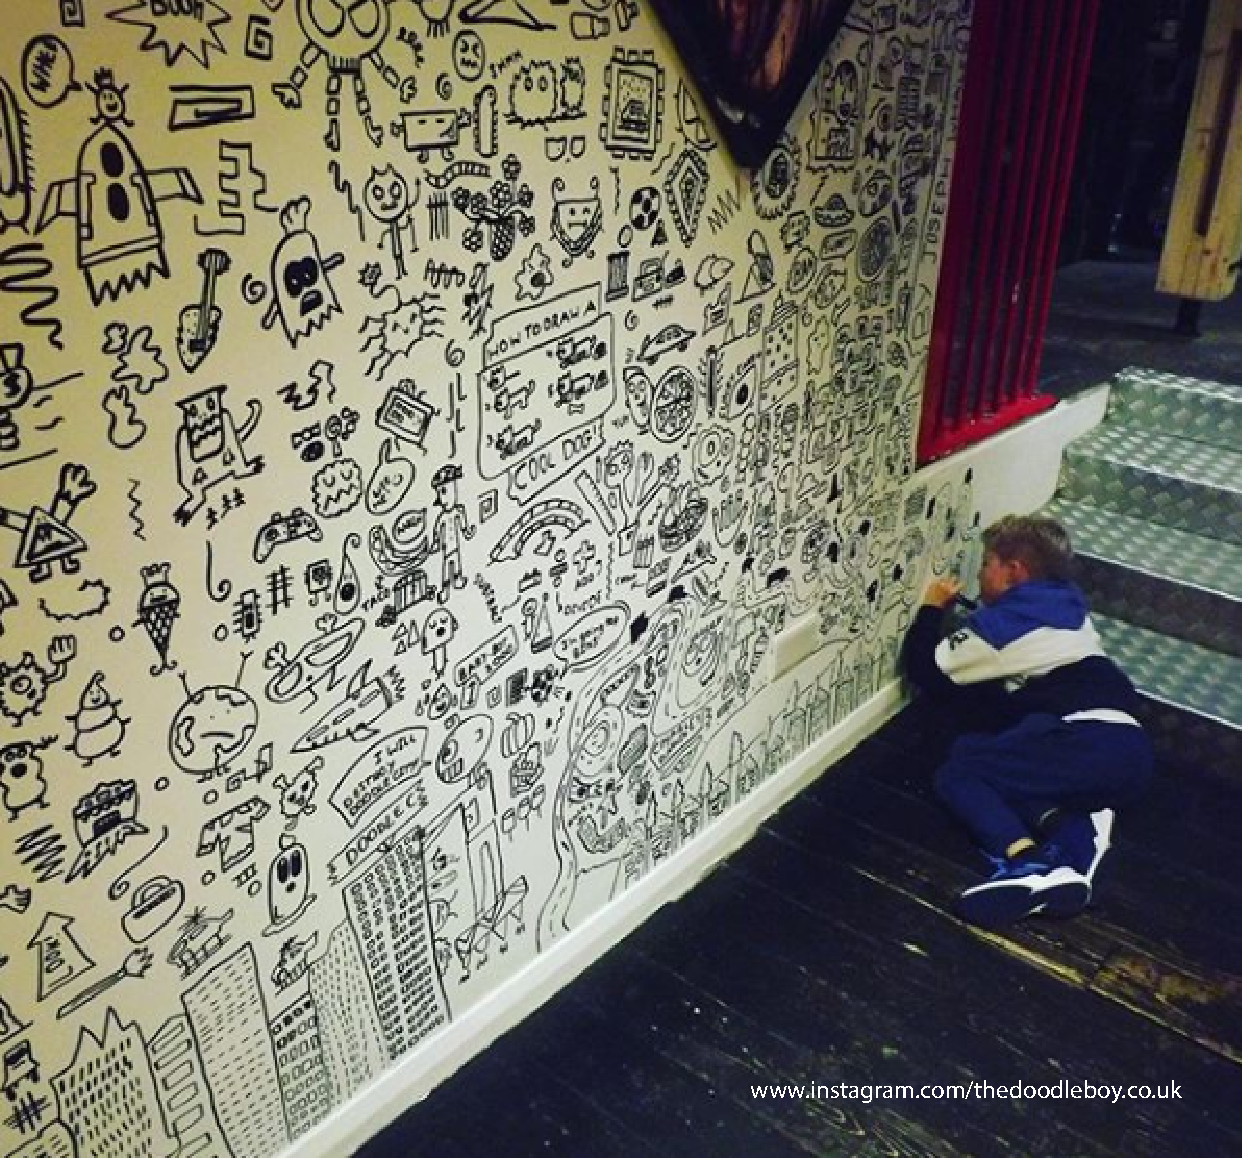
\includegraphics[width=0.5\textwidth]{figures/intro/doodle_boy.pdf} 
%\caption{\label{fig_doodle_boy} 
%Doodle boy. }
%\end{figure}

%\mynote{
%Thesis Statement (one or two sentences)
%\begin{packeditems}
%\item What is your thesis about and what have you done?
%\item If you have a hypothesis what is it?
%\item How will you test (prove/disprove) your hypothesis?
%\end{packeditems}
%}

%\mynote{align with boundary}

\newtext
{
A \textit{packing} is a composition of 2D geometric
\textit{elements} within a \textit{container} region in the plane.
Packings can communicate a relationship between a whole and the parts that make it up.
Elements are united to emphasize the shape of the container,
but each is large enough to be appreciated individually.
Packings are popular in logo design, graphic design, and art.
Elements are shapes like man-made objects, animals, plants, abstract, or geometric.
Figure~\ref{fig_logo_packing}a shows the Unilever logo,
which is a packing of elements arranged inside a ``U'' container.
}

\newtext
{
The subset of the container that does not belong to any element is
called \textit{negative space} (Figure~\ref{fig_logo_packing}b).
We can also define negative space as separation and gaps between elements.
The evenness of negative space plays an important role in  packings.  
The artist should arrange elements in a way that their boundaries interlock with each other,
causing the separation between neighbouring elements to become roughly the same everywhere.
After all, element interlocking is imperfect. It is not uncommon that 
the artist artfully placed small elements such as triangles or circles to reduce remaining large gaps,
see two examples in Figure~\ref{fig_graphic_designs}.
}
%Figure~\ref{fig_graphic_designs} shows two examples that contain small circle or triangle elements.

%The artist should align elements in a way that their boundaries interlock with each other.
%Unlike jigsaw puzzles that have perfect interlocking, 
%packings contain unused container space that does not belong to any element,
%which is called \textit{negative space} (Figure~\ref{fig_logo_packing}b).
%The more the elements interlock, the more even the negative space becomes.
%After all, element interlocking ends up imperfect, it is not uncommon that 
%the artist artfully placed small elements
%to eliminate remaining negative (Figure~\ref{fig_graphic_designs}X).

\newtext
{
Elements can also be oriented to follow certain directions for aesthetic reasons.
Figure~\ref{fig_graphic_designs}b is an ornamental packing
of long thin elements that are bent and oriented outward from the center of the torso to create a flow visual style.
Another example is shown in Figure \ref{fig_woodland}, which is a packing of leaves, each is oriented toward the center of the container.
On both examples, the flow visual style gives an impression of progression and movements.}

\newtext{There has been a moderate amount of past research in computer
graphics, particularly in the field of non-photorealistic rendering,
on the generation of packings, or mosaics.  
See Chapter~\ref{chapter_related_work} for specific examples.  
However,  most techniques pack elements via rigid transformations, leading to
uneven element distribution and overlaps.  
Jigsaw Image Mosaics~\cite{Kim2002} and collages based on the Pyramid of Arclength
Descriptor~\cite{Kwan2016} are \textit{data-driven}.
These techniques rely on a large library of elements, so that given an
area to fill in a partial composition, there is likely to be an
element in the library with a compatible shape.  The challenge is 
\textit{finding compatible elements},
which requires designing a shape matching technique that is fast and robust.
%The search space is enormous, since a single element
%can have many configurations through scaling or rotation.
Additionally, they cannot guarantee to find a compatible element
at every iteration, and elements typically do not fit perfectly with each other 
or the container boundary.
The remedy here is providing more data with increased computation time.
However, a large library may not be feasible or artistically desirable.
If an artist wants a packing of hand-drawn cats, and a data-driven approach 
cannot find a good result with ten cat shapes, 
the artist may not want to draw 100 or 1000 cats to ensure a better fit.
}

\newtext
{
In this thesis, we propose \textit{deformation-driven} methods.
Instead of finding compatible elements,
we intent to \textit{create compatible elements} through deformation
that can adapt to the shapes of neighboring elements and the container boundary.
We allow elements to deform in a controlled way,
to trade off between the evenness of the element distribution and 
the deformations of the individual elements.
By building an algorithm with a controllable deformation model at its core, we achieve a
more even distribution of negative space, even with a small library of element shapes.
}

\newtext
{
Deformation-driven methods also allow us to work toward a design principle called \textit{uniformity amidst variety}~\cite{Hutcheson1729, Gombrich}. 
\textit{Uniformity} aims for an overall unity of design and 
\textit{variety} seeks to break up the monotony of pure repetition.
We can achieve a degree of uniformity by using repeated copies of a small library of elements, but balance that uniformity with
variety by deforming those elements. 
We believe that there is a value in deformation that can generate plausible families of related elements from a single input shape.
}

\newtext
{
% https://learningenglish.voanews.com/a/the-more-i-practice-the-more-i-remember/4995040.html
The evenness of negative space is an indicator of the quality of a packing.
The more the elements interlock, the more even the negative space. % becomes
%Methods for measuring the evenness provide a quantitative means of evaluating
%and comparing packing algorithms.  
We are interested in quantitative measurements of the evenness 
in order to evaluate and compare packing algorithms.
In this paper we discuss several possible measurements of 
evenness based on methods from spatial statistics.
}

\newtext
{
In this thesis, our contribution is developing three deformation-driven packing methods and 2D packing quantitative metrics:
\begin{enumerate}
\item FLOWPAK is a packing method that deforms long thin elements to follow a user-defined vector field (Chapter~\ref{chapter_flowpak}).
\item RepulsionPak is a packing method that utilizes repulsion forces to distribute and deform elements,
	each is represented as a mass-spring system (Chapter~\ref{chapter_repulsionpak}).
\item AnimationPak is a method to pack 2D animated elements inside a static 2D container. 
	Each element is an extruded 3D shape in a spacetime domain 
	and we view the animated packing problem as a 3D packing in that domain.
	(Chapter~\ref{chapter_animationpak}). 
\item  Quantitative metrics for measuring the evenness of negative space: spherical contact probabilities,
histograms of the distance transforms, and the overlap functions (Chapter~\ref{chapter_qualitative_metrics}). 
\end{enumerate}
}


%\begin{labeling}{alligator}
%\item [ant] really busy all the time
%\item [chimp] likes bananas
%\item [alligator] very dangerous animal, sharp teeth, long
%muscular tail and a bit of text that is longer than one
%line and shows the alignment of text quite nicely
%\end{labeling}


%\mynote{TODO: Copy from comp\_2}
%A \textit{packing} is an arrangement of 2D geometric
%\textit{elements} within a \textit{container} region in the plane.
%Packings are popular in art, ornamentation, and graphics design.
%Figure ~\ref{fig_logo_packings}\ref{fig_graphics_designs}\ref{fig_woodland}\ref{fig_valve_lobby}\ref{fig_doodle_boy} show several packing examples.
%They can effectively convey a relationship between a unified whole (the
%container shape) and its many sub-parts (the elements).

%\mynote{maybe put negative space to the background section}
%Elements are shapes like animals,
%plants, geometric forms, or man-made objects.
%An artist distributes elements so that they communicate
%the shape of the container. 
%The subset of the container that does not belong to any element is
%called \textit{negative space}
%(Fig.~\ref{packing_example}, right).
%We can also interpret negative space as separation and gaps between elements.
%The evenness of negative space plays an important role in 
%packings.  
%The artist should arrange elements in a way that their boundaries interlock with each other,
%causing the separation between neighbouring elements to become roughly the same everywhere.
%As the elements in a packing become perfectly interlocked,
%the packing turns into a \textit{tiling}: a set of elements that exactly
%fill a container with no overlaps and no negative space (Fig.~\ref{related_work_images}b).



%\mynote{Motivation, Why is this problem you've worked on important}
%\mynote{Goals / Objectives, What are you trying to do and why? 
%How will you or the reader know if or when you've met your objectives?}


%\mynote{
%Contributions, What is new, different, better, significant? Why is the world a better place because of what you've done? What have you contributed to the field of research?  What is now known/possible/better because of your thesis?
%}



%\mynote {Explain briefly FLOWPAK, RepulsionPak, and AnimationPak.}